		\subsection{Metodología de las mediciones}
			
		Para calcular la absorción sonora se deben medir los tiempos de reverberación siguiendo el procedimiento de la Norma IRAM $4065/1995$ \textit{Acústica. Medición de absorción de sonido en sala reverberante}.\\

		La sala reverberante utilizada posee un volumen de \SI{189}{\cubic\meter}, una superficie interior de \SI{208}{\square\meter}, y cumple con los requisitos de estas normas.\\

		Durante el ensayo se utilizan 2 posiciones diferentes de las fuentes sonoras y 6 posiciones del micrófono, realizándose 3 registros por cada combinación fuente-micrófono. De este modo, cada tiempo de reverberación es el resultado del promedio de 36 caídas. Este procedimiento se lleva a cabo para dos condiciones: la cámara vacía y la cámara con la muestra ensayada en su interior.\\

		Con los tiempos de reverberación medidos, se calcula el coeficiente de absorción sonora \texttt{$\alpha_s$} (adimensional), para las bandas de tercios de octava comprendidas entre $100$ y \SI{5000}{\Hz}; finalmente, a partir del \texttt{$\alpha_s$}, se obtiene el valor del índice de evaluación de la absorción sonora \texttt{$DL_{\alpha}$}, cuya expresión se analizará en la subsección correspondiente.
		
		\subsection{Valores medidos}
		
		Los paneles se colocaron sobre el piso de la cámara reverberante, con su cara fonoabsorbente hacia arriba, expuesta al sonido, como se muestra en la Figura \ref{2_camara}.\\
		
		\begin{figure}[H]
			\centering
			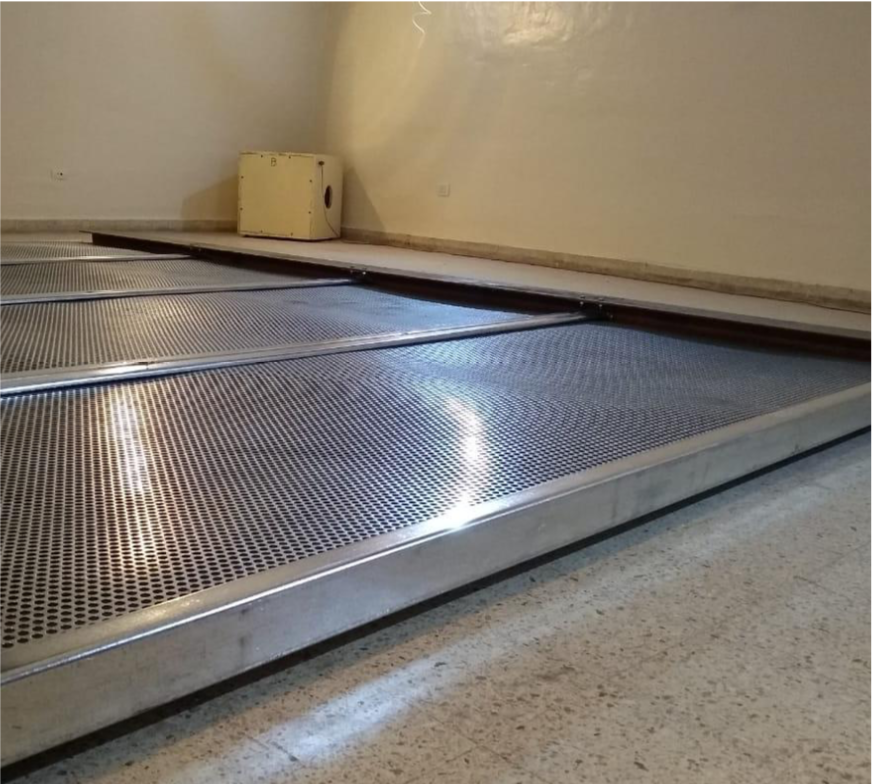
\includegraphics[scale=0.50]{2_camara.png}\\
			\caption{Montaje de ensayo en cámara reverberante.}
			\label{2_camara}
		\end{figure}
		
		En la Tabla de la Figura \ref{2_mediciones} se presentan los valores de tiempos de reverberación medidos para las distintas condiciones de ensayo.\\
		
		\begin{figure}[H]
			\centering
			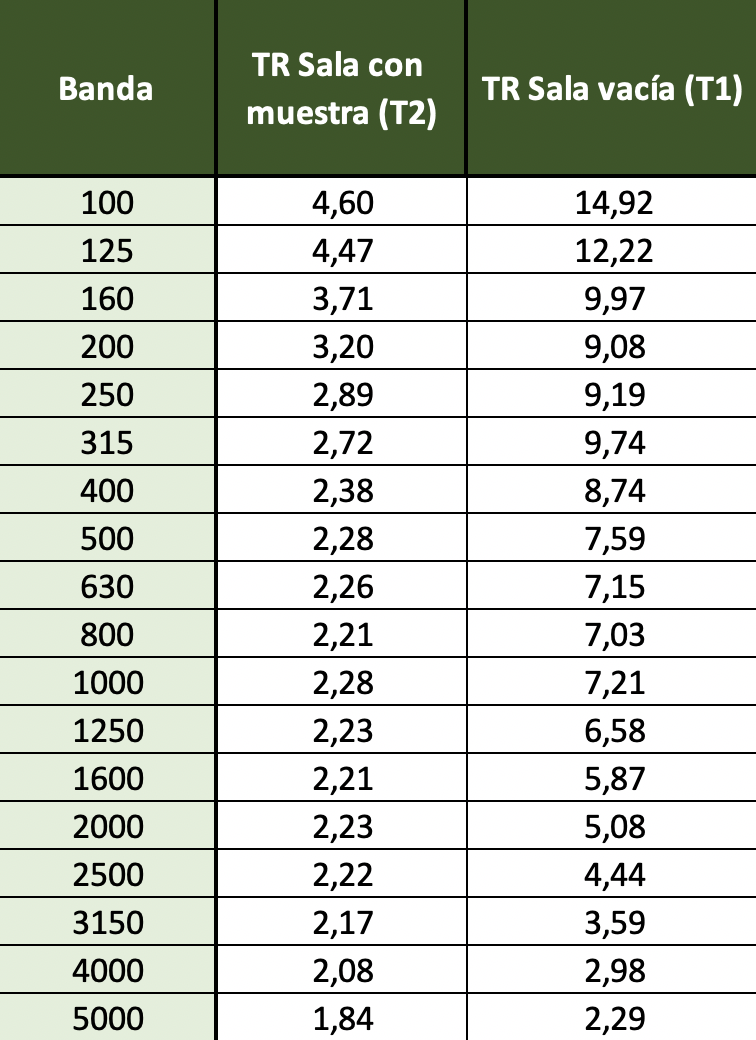
\includegraphics[scale=0.50]{2_mediciones.png}\\
			\caption{Tiempos de reverberación medidos, en segundos.}
			\label{2_mediciones}
		\end{figure}
		
		Se constató que la temperatura y la humedad permanecieran constantes durante el ensayo, y los valores registrados fueron: \SI{26.7}{\celsius} y $62\,\%$, respectivamente.\\
		
		\subsection{Análisis de las mediciones}
		
		Las mediciones del tiempo de reverberación de la sala se muestran en el siguiente gráfico:

		\begin{figure}[H]
			\centering
			\includegraphics[scale=0.60]{2_gráfico_tr.png}\\
			\caption{Tiempos de reverberación de la sala con y sin la muestra.}
			\label{2_gráfico_tr}
		\end{figure}
		
		Observando ambas curvas, se puede notar que el tiempo de reverberación baja considerablemente ante la colocación de la muestra en la sala. La sala vacía cuenta con un tiempo de reverberación que varía desde los $14.92$ segundos (aproximadamente) para las frecuencias más bajas, hasta los $2.29$ segundos para las frecuencias más altas, lo que representa un parámetro muy variable. Al colocar la muestra, este tiempo no sólo se logra disminuir hasta en un $70 \%$ para algunas frecuencias (para $100$ Hz y $315$ Hz, por ejemplo), sino que también se lo puede apreciar con un carácter más constante a lo largo de cada banda, acotando su valor entre un mínimo de $1.84$ segundos y un máximo de $4.60$ segundos.\\
		
		Para proceder a obtener el coeficiente de absorción, se debe calcular antes el parámetro del årea equivalente de absorción del material, en $m^2$:
		
		\begin{equation}
			A_{eq} = 55.3 \, \frac{V}{c} \, \left(\frac{1}{TR_1} - \frac{1}{TR_2}\right)
		\end{equation}
		
		La velocidad del sonido varía con la temperatura según \texttt{c = 332 + 0.608\,T}. Usando el dato mencionado de \texttt{T = \SI{26.7}{\celsius}}, se calcula \texttt{c = \SI{348.23}{\meter/\second}}. \texttt{$V$} es el dato del volumen de la cámara utilizada (\SI{189}{\cubic\meter}). \texttt{$TR_1$} y \texttt{$TR_2$} es el tiempo de reverberación de la cámara vacía y con la muestra, respectivamente, para cada banda de frecuencias.\\
		
		Finalmente, el coeficiente de absorción del material en función de la frecuencia es:
		
		\begin{equation}
			\alpha_s = \frac{A_{eq}}{S}
		\end{equation}
		
		S es el valor de la superficie del material a caracterizar; en este caso: \texttt{S = \SI{10}{\cubic\meter}}.\\

		A partir del cálculo de las expresiones anteriores con los datos medidos, se obtiene el coeficiente de absorción sonora para cada banda de tercios de octava de frecuencia.

		\begin{figure}[H]
			\centering
			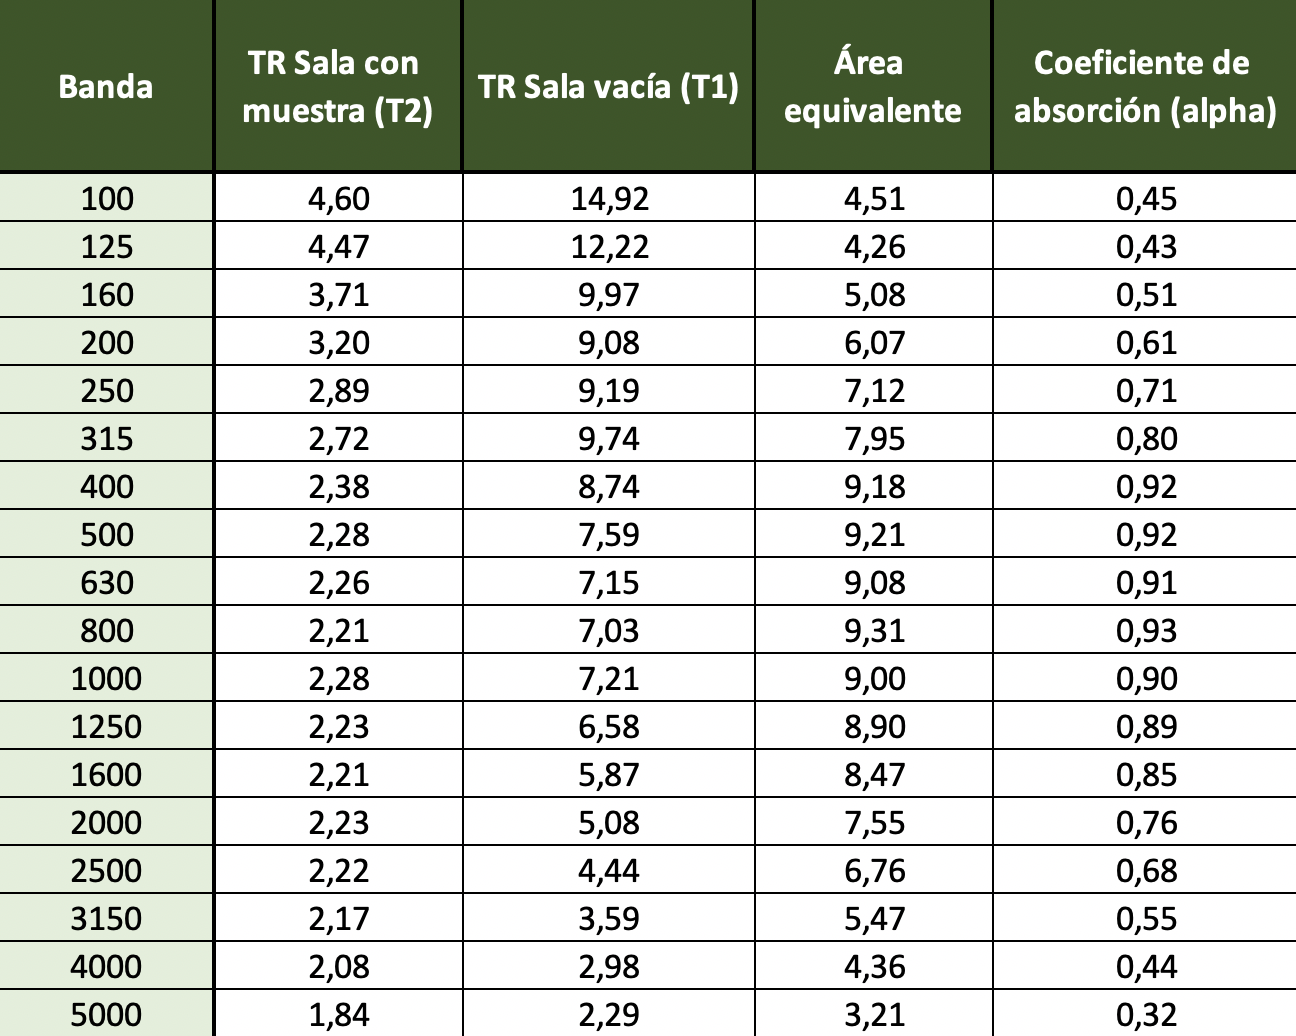
\includegraphics[scale=0.50]{2_tabla_final.png}\\
			\caption{Datos numéricos obtenidos para el coeficiente de absorción para cada banda de frecuencia.}
			\label{2_tabla_final}
		\end{figure}
		
		Los resultados se exponen en el siguiente gráfico, cuyos datos son los de la tabla \ref{2_tabla_final}:

		\begin{figure}[H]
			\centering
			\includegraphics[scale=0.60]{2_gráfico_absorción.png}\\
			\caption{Coeficiente de absorción para cada banda de frecuencia.}
			\label{2_gráfico_absorción}
		\end{figure}
		
		Observando el gráfico de la Figura \ref{2_gráfico_absorción}, se puede concluir en que el material absorbe \textit{casi} la totalidad del sonido (más del $90 \%$) para las frecuencias comprendidas entre los $	400$ y $1250$ Hz. Para frecuencias fuera de ese rango, absorbe entre un $32 \%$ y un $85 \%$.
		
		\subsection{Índice de evaluación de la absorción sonora ($D\,L_\alpha$)}
		
		A partir de los valores del coeficiente de absorción sonora $\alpha_s$ dependientes de la frecuencia, y siguiendo los lineamientos de la norma \texttt{IRAM 4065/1995}: \textit{Acústica. Medición de absorción de sonido en sala reverberante}, se obtiene el número global: este índice es calculado como la diferencia de niveles de presión sonora ponderados A, mediante la siguiente ecuación, expresada en decibeles, y se redondea al entero más próximo:
	
		\begin{equation}
			DL_{\alpha} = -10\,log\left(1- \frac{\sum \alpha_{s\,i}\,10^{0.1\,L_i}}{\sum 10^{0.1\,L_i}}\right)
		\end{equation}
	
		Donde:
		\begin{itemize}
			\item $\alpha_{s\,i}$: Coeficiente de absorción sonora de la i-ésima banda de tercio de octava;
			\item $L_i$: Nivel de presión sonora de ruido normalizado ponderado A, en dB, de la i-ésima banda de tercio de octava del ruido normalizado que corresponda utilizar.
		\end{itemize}
		
		\begin{align}
			DL_{\alpha} &= -10\,log\left(\frac{\sum 10^{0.1\,L_i} - \sum \alpha_{s\,i}\,10^{0.1\,L_i}}{\sum 10^{0.1\,L_i}}\right)\\
			DL_{\alpha} &= 10\,log\left(\sum 10^{0.1\,L_i}\right) - 10\,log\left(\sum 10^{0.1\,L_i} - \sum \alpha_{s\,i}\,10^{0.1\,L_i}\right)
		\end{align}
			
		Observando la última expresión, se puede decir que este índice corresponde a una resta energética entre el nivel de presión sonora de ruido normalizado ponderado A y el sonido absorbido por el material en cuestión. Luego vemos los casos límites:
		
		\begin{itemize}
			\item Si el coeficiente de absorción se acerca a $0$, el índice tenderá a valer 0;
			\item Si el coeficiente de absorción tiende a $1$, el argumento del logaritmo del segundo termino tiende a 0, lo que lleva a un índice que tiende a infinito.
		\end{itemize}
		
		Teniendo en cuenta el espectro normalizado para el ruido de tráfico, se calcula siguiendo la expresión dada y se obtiene un valor de \texttt{$7.35$ dB}, que se debe redondear a:
		
		\begin{equation*}
			\boxed{DL_{\alpha} = 7 dB}
		\end{equation*}
			
		Para el caso del ruido ferroviario, el cálculo es de \texttt{$6.48 dB$}, que se debe redondear a:

		\begin{equation*}
			\boxed{DL_{\alpha} = 6 dB}
		\end{equation*}	
		
		\subsection{Clasificación del comportamiento de absorción}
		
		De acuerdo con lo establecido en la citada norma, las categorías normalizadas en función de $D\,L_\alpha$ son:

		\begin{table}[h!]
			\centering
			\begin{tabular}{cc}
			\toprule
			\textbf{Categoría} & \textbf{$DL_{\alpha}$ (dB)}\\
			\midrule
			$A_0$ & No determinado\\
			$A_1$ & $DL_{\alpha}$ < 4 \\
			$A_2$ & 4 a 7 \\
			$A_3$ & 8 a 11 \\
			$A_4$ & 12 a 15 \\
			$A_5$ & $DL_{\alpha}$ > 15 \\
			\bottomrule
			\end{tabular}
		\end{table}
		
		Ambos valores obtenidos para el índice $DL_{\alpha}$ se encuentran en la categoría \texttt{categoría A2}. Este resultado \textbf{no} cumple con la especificación buscada para el aislamiento acústico. Para cumplir con la especificación, el $DL_{\alpha}$ calculado debía estar entre los $8$ y $11$ dB.

